% =============================================================
%  wepe_direction_compare.tex
%  编译说明（Overleaf 必读）：
%    1) 推荐 XeLaTeX：Menu -> Compiler -> XeLaTeX
%       中文用 ctex 渲染，效果最好（标题/粗体/标点）
%    2) 如不切换编译器（默认 pdfLaTeX），也能编译：
%       中文用 CJKutf8 兜底；公式粗体略简化但内容正确
%  本文件已用 \ifPDFTeX 自动判断，无需手动改
% =============================================================
\documentclass[11pt]{article}

% ---------- 引擎判断：根据编译器自动切换中文包 ----------
\usepackage{iftex}
\ifPDFTeX
  % pdfLaTeX 分支：用 CJK 兜底
  \usepackage{CJKutf8}
  \newcommand{\zh}[1]{\begin{CJK}{UTF8}{gbsn}#1\end{CJK}}
\else
  % XeLaTeX / LuaLaTeX 分支：用 ctex
  \usepackage[UTF8, scheme=plain]{ctex}
  \newcommand{\zh}[1]{#1}
\fi

% ---------- 其他宏包（两个引擎通用） ----------
\usepackage{graphicx}
\usepackage{subcaption}
\usepackage{booktabs}
\usepackage{geometry}
\usepackage{amsmath}
\usepackage{float}
\usepackage{xcolor}
\geometry{a4paper, margin=2.3cm}

% 图片相对路径（与本 tex 同目录下的 figures/ 文件夹）
\graphicspath{{figures/}}

\title{\zh{\textbf{MEEF 控制点移动方向对比：\\ 角平分线 (bisector) vs.\ X/Y 解耦 (xy)}}}
\author{\zh{Litho Simulation 课题组}}
\date{\today}

\begin{document}
\maketitle

% pdfLaTeX 路径下需要一次性进入 CJK 环境
\ifPDFTeX\begin{CJK}{UTF8}{gbsn}\fi

\begin{abstract}
\zh{本文对比 MEEF 控制点优化中两种移动策略——\textbf{角平分线一维位移 (bisector)} 与
\textbf{X/Y 两方向解耦的二维位移 (xy)}——在两套实验设置下的优化效果。
分别给出两种策略在 wEPE 最优时刻的掩模 (mask)、晶圆成像 (wafer image, WI)，
以及二者在迭代过程中的 wEPE 损失函数收敛曲线，并据此分析各策略的优劣。
两套实验为：\textbf{(I) DPS 直接参数化优化（工字型图案）} 与
\textbf{(II) MEEF Pipeline（matrix\_0525，含 SRAF）}。}
\end{abstract}

%======================================================================
\section{\zh{对比方法说明}}
%======================================================================
\begin{itemize}
  \item \zh{\textbf{bisector（角平分线）}：沿每个控制点相邻边的角平分线方向做\emph{一维}位移，
        仅构建单一 MEEF 矩阵 $M$，TSVD 求解得到每个控制点沿角平分线的标量位移 $\Delta d$。}
  \item \zh{\textbf{xy（X/Y 解耦）}：分别构建 $X$ 方向矩阵 $M_x$ 与 $Y$ 方向矩阵 $M_y$，
        各自 TSVD 求解得到 $\Delta x$、$\Delta y$，再合成出真实的二维移动向量
        $\Delta \mathbf{r}=(\Delta x,\Delta y)$，自由度更高。}
\end{itemize}

\zh{评价指标}：
\[
  \text{EPE} = \frac{1}{N_{ep}}\sum_i |d_i|,\qquad
  \text{wEPE} = \frac{\sum_i w_i\,|d_i|}{\sum_i w_i},
\]
\zh{其中 $d_i$ 为第 $i$ 个评估点的边缘放置误差，$w_i$ 为权重；wEPE 越小代表加权边缘控制越好。}

%======================================================================
\section{\zh{实验 I：DPS 直接参数化优化（工字型图案）}}
%======================================================================

\subsection{\zh{wEPE 最优掩模与晶圆成像}}

\begin{figure}[H]
  \centering
  \begin{subfigure}[t]{0.45\textwidth}
    \centering
    
\includegraphics[width=\linewidth]{dps_bisector_mask.png}
    \caption{\zh{bisector — 掩模}}
  \end{subfigure}\hfill
  \begin{subfigure}[t]{0.45\textwidth}
    \centering
    
\includegraphics[width=\linewidth]{dps_bisector_wafer.png}
    \caption{\zh{bisector — 晶圆成像 (WI)}}
  \end{subfigure}

  \vspace{0.6em}

  \begin{subfigure}[t]{0.45\textwidth}
    \centering
    
\includegraphics[width=\linewidth]{dps_xy_mask.png}
    \caption{\zh{xy — 掩模}}
  \end{subfigure}\hfill
  \begin{subfigure}[t]{0.45\textwidth}
    \centering
    
\includegraphics[width=\linewidth]{dps_xy_wafer.png}
    \caption{\zh{xy — 晶圆成像 (WI)}}
  \end{subfigure}
  \caption{\zh{实验 I：bisector 与 xy 策略在 wEPE 最优时刻的掩模与晶圆成像对比。}}
\end{figure}

\subsection{\zh{损失函数（wEPE 收敛曲线）}}

\begin{figure}[H]
  \centering
  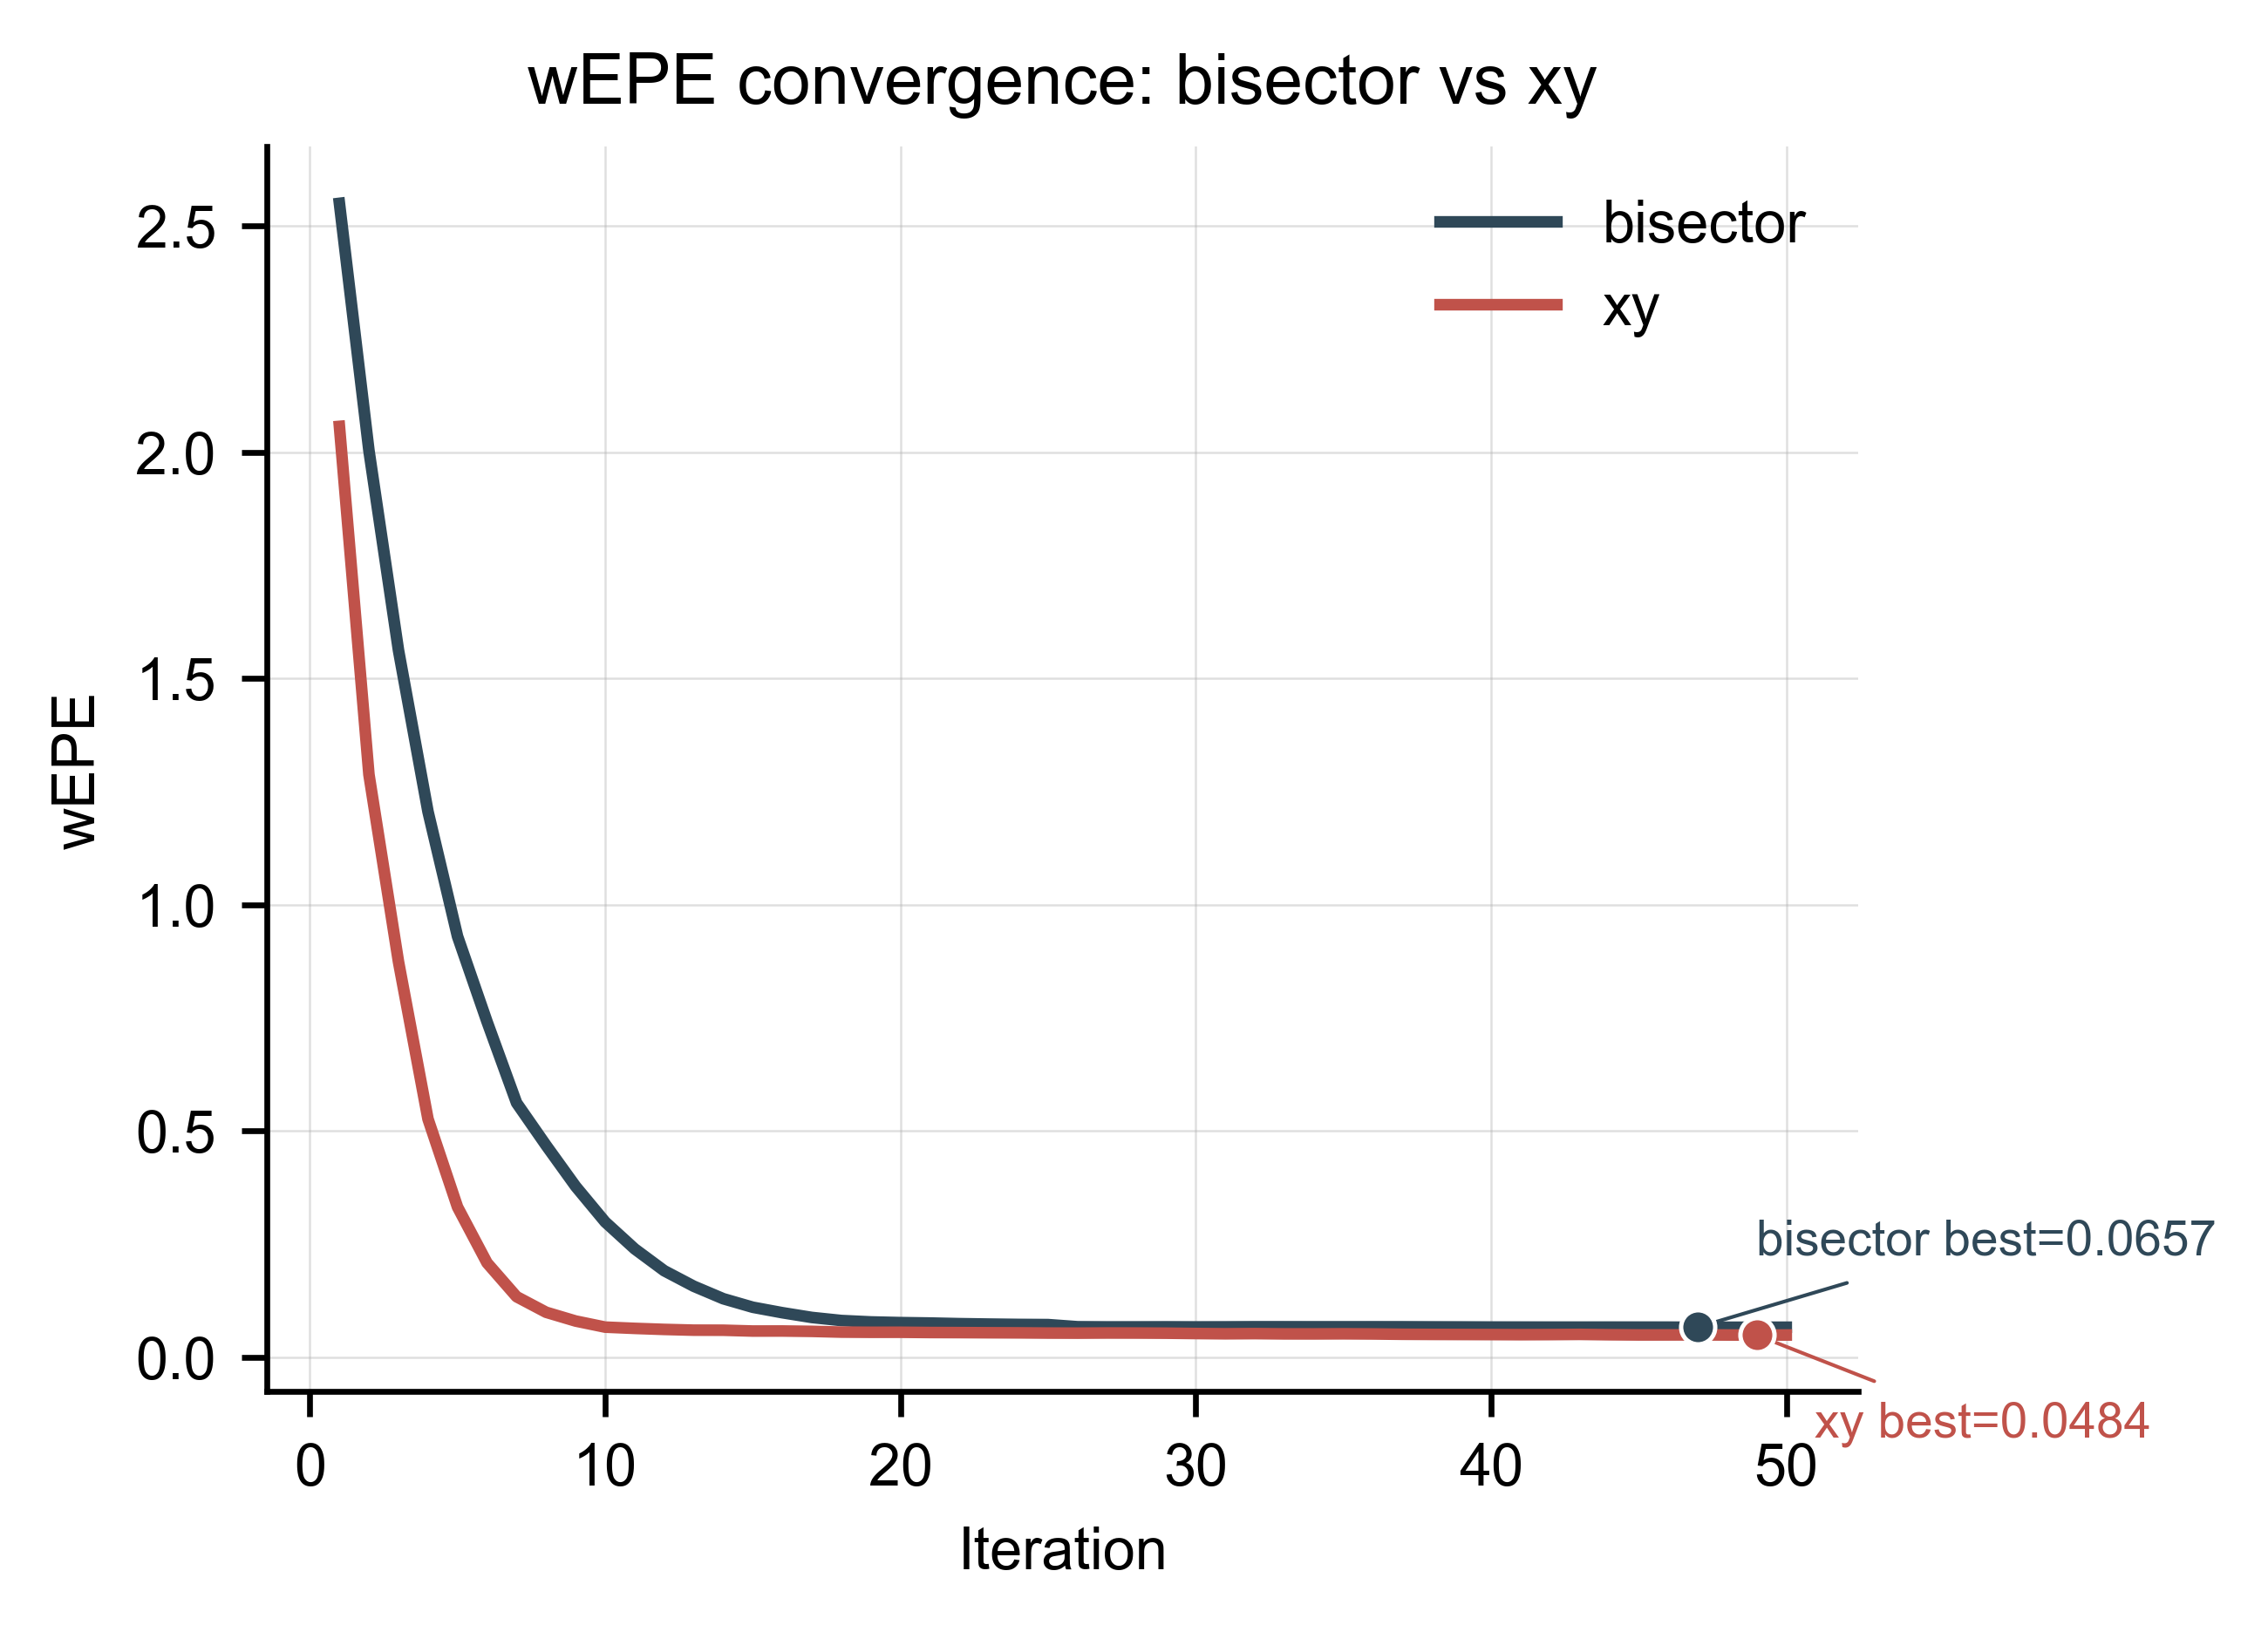
\includegraphics[width=0.78\textwidth]{loss_dps.png}
  \caption{\zh{实验 I：bisector vs.\ xy 的 wEPE 收敛曲线。
           bisector 最优 $=0.0657$，xy 最优 $=0.0484$。}}
\end{figure}

\subsection{\zh{结果数据}}

\begin{table}[H]
  \centering
  \caption{\zh{实验 I（工字型）最优结果对比}}
  \begin{tabular}{lccc}
    \toprule
    \zh{移动策略} & \zh{最优迭代} & EPE & wEPE \\
    \midrule
    bisector & 47 & 0.0672 & 0.0657 \\
    \textbf{xy} & 49 & \textbf{0.0469} & \textbf{0.0484} \\
    \midrule
    \zh{相对改善} & --- & $\downarrow$ 30.2\% & $\downarrow$ 26.3\% \\
    \bottomrule
  \end{tabular}
\end{table}

%======================================================================
\section{\zh{实验 II：MEEF Pipeline（matrix\_0525，含 SRAF）}}
%======================================================================

\subsection{\zh{wEPE 最优掩模与晶圆成像}}

\begin{figure}[H]
  \centering
  \begin{subfigure}[t]{0.45\textwidth}
    \centering
    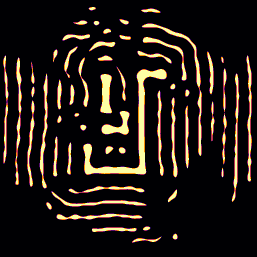
\includegraphics[width=\linewidth]{pipe_bisector_mask.png}
    \caption{\zh{bisector — 掩模}}
  \end{subfigure}\hfill
  \begin{subfigure}[t]{0.45\textwidth}
    \centering
    
\includegraphics[width=\linewidth]{pipe_bisector_wafer.png}
    \caption{\zh{bisector — 晶圆成像 (WI)}}
  \end{subfigure}

  \vspace{0.6em}

  \begin{subfigure}[t]{0.45\textwidth}
    \centering
    
\includegraphics[width=\linewidth]{pipe_xy_mask.png}
    \caption{\zh{xy — 掩模}}
  \end{subfigure}\hfill
  \begin{subfigure}[t]{0.45\textwidth}
    \centering
    
\includegraphics[width=\linewidth]{pipe_xy_wafer.png}
    \caption{\zh{xy — 晶圆成像 (WI)}}
  \end{subfigure}
  \caption{\zh{实验 II：bisector 与 xy 策略在 wEPE 最优时刻的掩模与晶圆成像对比。}}
\end{figure}

\subsection{\zh{损失函数（wEPE 收敛曲线）}}

\begin{figure}[H]
  \centering
  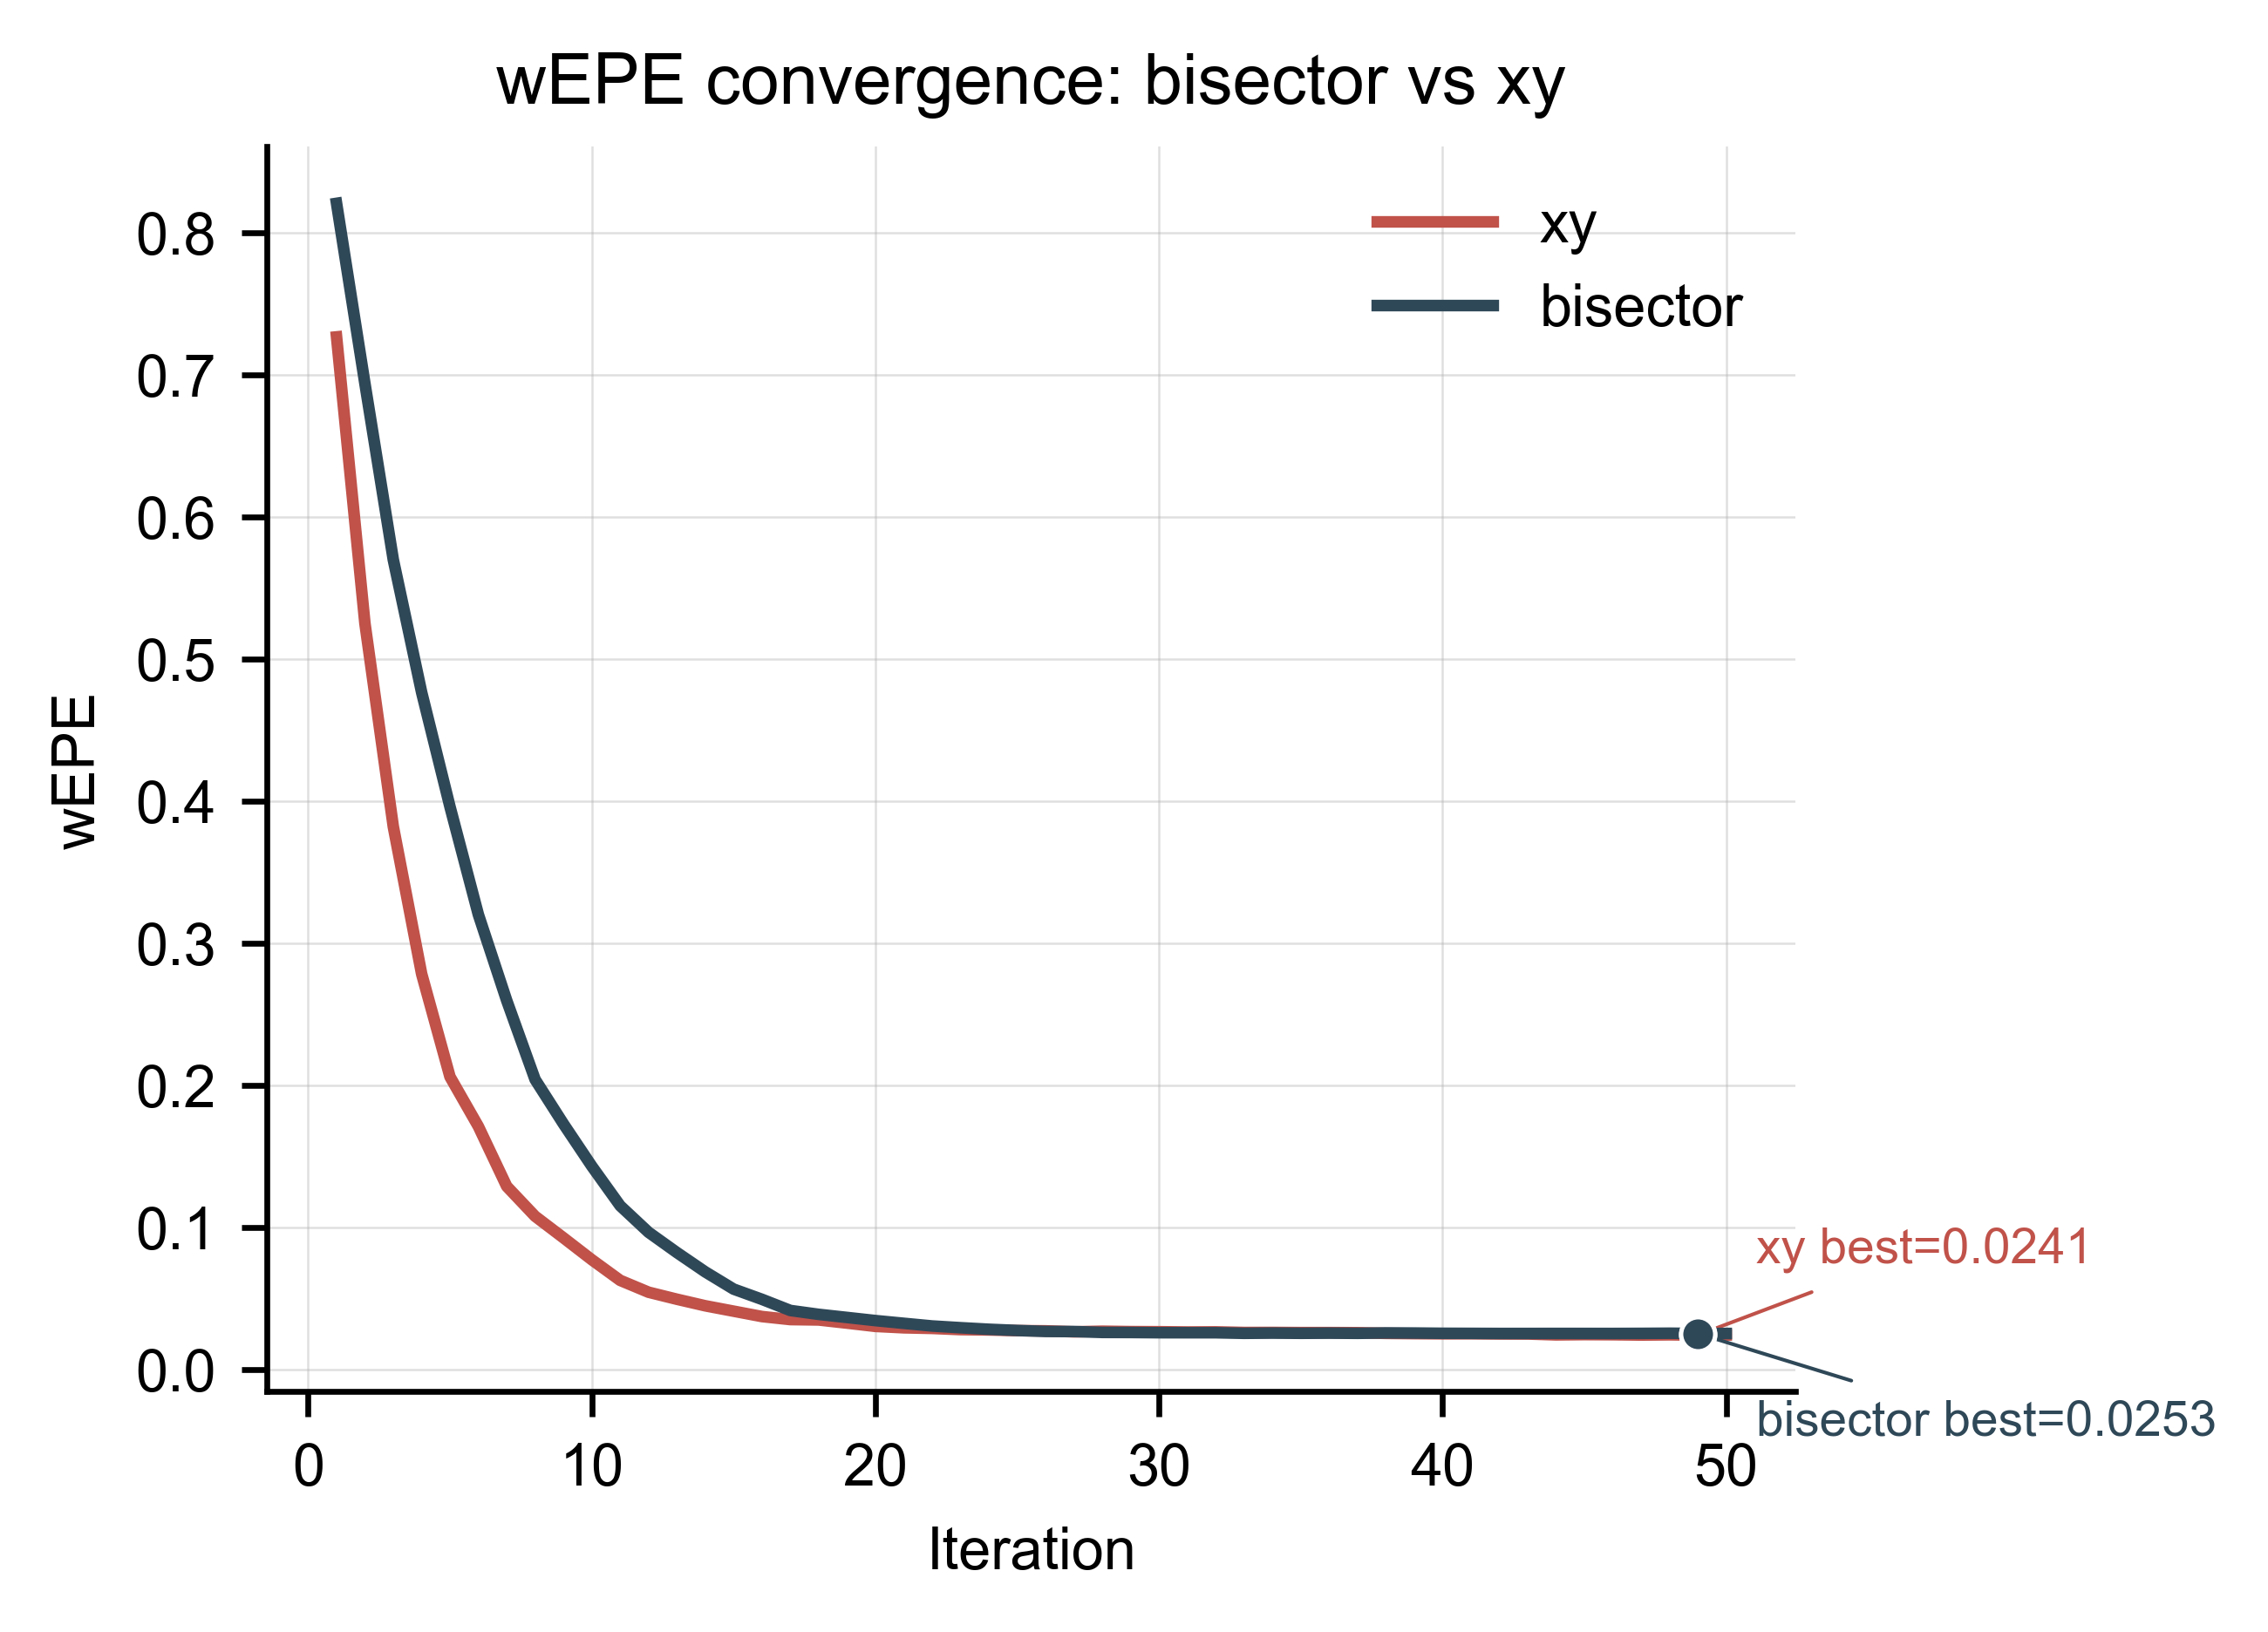
\includegraphics[width=0.78\textwidth]{loss_pipe.png}
  \caption{\zh{实验 II：bisector vs.\ xy 的 wEPE 收敛曲线。
           xy 最优 $=0.0241$，bisector 最优 $=0.0253$。}}
\end{figure}

\subsection{\zh{结果数据}}

\begin{table}[H]
  \centering
  \caption{\zh{实验 II（matrix\_0525 pipeline）最优结果对比}}
  \begin{tabular}{lccc}
    \toprule
    \zh{移动策略} & \zh{最优迭代} & EPE & wEPE \\
    \midrule
    bisector & 46 & 0.0433 & 0.0253 \\
    \textbf{xy} & 49 & \textbf{0.0313} & \textbf{0.0241} \\
    \midrule
    \zh{相对改善} & --- & $\downarrow$ 27.7\% & $\downarrow$ 4.7\% \\
    \bottomrule
  \end{tabular}
\end{table}

%======================================================================
\section{\zh{损失函数分析与结论}}
%======================================================================

\subsection{\zh{收敛行为分析}}
\begin{itemize}
  \item \zh{\textbf{收敛速度}：在两套实验中，\textbf{xy 策略前期下降都更快}。实验 I 中
        xy 起点更低（$\approx 2.06$ vs.\ bisector $\approx 2.55$）且在第 10 次迭代附近
        已基本进入平台区；bisector 则需到第 15$\sim$20 次才趋于平稳。这说明二维自由度
        让每次迭代的可行下降方向更充分，单步降幅更大。}
  \item \zh{\textbf{最终精度}：两套实验中 xy 的最终 wEPE 均不劣于 bisector。
        实验 I 优势显著（wEPE $0.0484$ vs.\ $0.0657$，相对降低约 $26\%$）；
        实验 II 二者非常接近（wEPE $0.0241$ vs.\ $0.0253$，相对降低约 $5\%$）。}
  \item \zh{\textbf{稳定性}：两种策略在约 20 次迭代后都进入平稳平台，无明显振荡或发散，
        表明 TSVD 截断与权重加权使两种线性化求解均数值稳定。}
\end{itemize}

\subsection{\zh{两套实验差异的原因}}
\begin{itemize}
  \item \zh{实验 I（DPS，无 SRAF）的图形以工字型主体边缘为主，控制点的最优位移方向
        往往\emph{不与角平分线对齐}，因此放开 X/Y 解耦带来的增益明显（$\sim26\%$）。}
  \item \zh{实验 II（pipeline，含 SRAF，$k=5$）经 LSM 初始化后掩模已较接近最优，
        角平分线方向已能较好近似真实位移方向，故 xy 的额外自由度收益被压缩到 $\sim5\%$，
        但仍保持小幅领先且收敛更快。}
\end{itemize}

\subsection{\zh{总体结论}}
\begin{enumerate}
  \item \zh{\textbf{X/Y 解耦 (xy) 策略整体优于角平分线 (bisector) 策略}：
        在两套实验中均取得更低或相当的 EPE/wEPE，且前期收敛更快。}
  \item \zh{\textbf{增益大小依赖图形与初始化质量}：当目标图形边缘方向复杂、或初始掩模
        离最优较远时（实验 I），xy 的二维自由度优势显著；当已有良好初始化（实验 II）时，
        二者趋于接近，但 xy 仍小幅领先。}
  \item \zh{\textbf{实践建议}：在可接受约 2 倍 MEEF 矩阵构建开销（需分别求 $M_x$、$M_y$）的前提下，
        推荐默认采用 \textbf{xy} 策略以获得更快收敛与更低残差；对计算资源敏感、
        且图形规整、初始化良好的场景，bisector 仍是高性价比的备选。}
\end{enumerate}

% pdfLaTeX 路径下需要配对结束 CJK 环境
\ifPDFTeX\end{CJK}\fi

\end{document}
